%\newpage
\chapter{Examples} \label{Exampleschap}
%\section{Examples}

\section{General methodology}
A simulation of GISAXS using \BornAgain\ platform can be decomposed into the following points:
\begin{itemize}
\item Definition of the materials by specifying their names and their
  refractive indices,
\item Definition of particles: shapes, sizes, refractive indices of
  the constituting material, interference functions,
\item Definition of the layers: thicknesses, roughnesses, associations with the previously defined
materials,
\item Inclusion of the particles in layers: \textbf{density or proportion}, positions, orientations, 
\item Assembling the sample: generation of a multilayered system,
\item Specifying the input beam and the output detector's
  characteristics,
\item Running the simulation,
\item Saving the data.
\end{itemize}

\noindent The sample is built from object oriented building blocks instead of loading data files.

\section{Conventions}

\subsection{Geometry of the sample}

\noindent The geometry used to describe the sample is shown in
Fig.~\ref{fig:multil3d}. The $z$-axis is perpendicular to the sample's
surface and pointing upwards. The $x$-axis  is perpendicular to the
plane of the detector and the $y$-axis is along it. The input and the scattered output beams are each by two angles
$\alpha_0$, $\phi_0$ and $\alpha_f$, $\phi_f$ respectively. Then for each other layer
$j=1,..., N-1$, the incident angles $\alpha_j$ and $\phi_j$  are defined with
respect to the bottom of the layer. Our choice of orientation for the
angles $\alpha_j$ is so that $\alpha_0$ and $\alpha_f$ shown in fig.~\ref{fig:multil3d}  are positive. \\


\noindent The layers are defined by their thicknesses (parallel to the
$z$-direction), their possible
roughnesses (equal to 0 by default) and the refractive index of the
material. We do not define any dimensions in the $x$, $y$
directions. And, except for roughness, the layer's vertical boundaries are plane and
perpendicular to the $z$-axis. There is also no limitation to the
number of layers that could be defined in \BornAgain.\\

\noindent {\huge\danger} 
\colorbox{Lightgray}{\parbox{\dimexpr\linewidth-8\fboxsep}
{\underline{Remark} - Order of the different steps for the simulation: \\
When assembling the sample, the layers are defined from top to
bottom. So in most cases the first layer will be the air layer.}}\\

\noindent The particles are characterized by their form factors (\textit{i.e.} the Fourier transform of the shape function - see the list of form factors implemented
  in \BornAgain) and
the refractive index of the composing material. The number of input parameters for the form
  factor depends on the
  particle symmetry; it ranges from one parameter for a sphere (its
  radius) to three for an ellipsoid (its three main axis lengths).\\ By
  placing the particles
inside or on top of a layer, we impose their vertical positions. The in-plane distribution of particles is linked with the way the
particles interfere with each other, which is therefore implemented
when dealing with the interference function. \\

\noindent {\huge\danger} 
\colorbox{Lightgray}{\parbox{\dimexpr\linewidth-8\fboxsep}
{\underline{Remark -} Depth of particles\\
The vertical positions of particles in a layer are given in relative
coordinates. For the top layer, the bottom corresponds to
\texttt{depth}=0. But for all the other layers, it is the top of the
layer which corresponds to \texttt{depth}=0.}}\\


\noindent The complex refractive index associated with a layer or a particle is written as $n=1-\delta +i\beta$, with
$\delta, \beta \in \mathbb{R}$. In our program we input $\delta$ and
$\beta$ directly. \\


\begin{figure}[h]
  \centering
    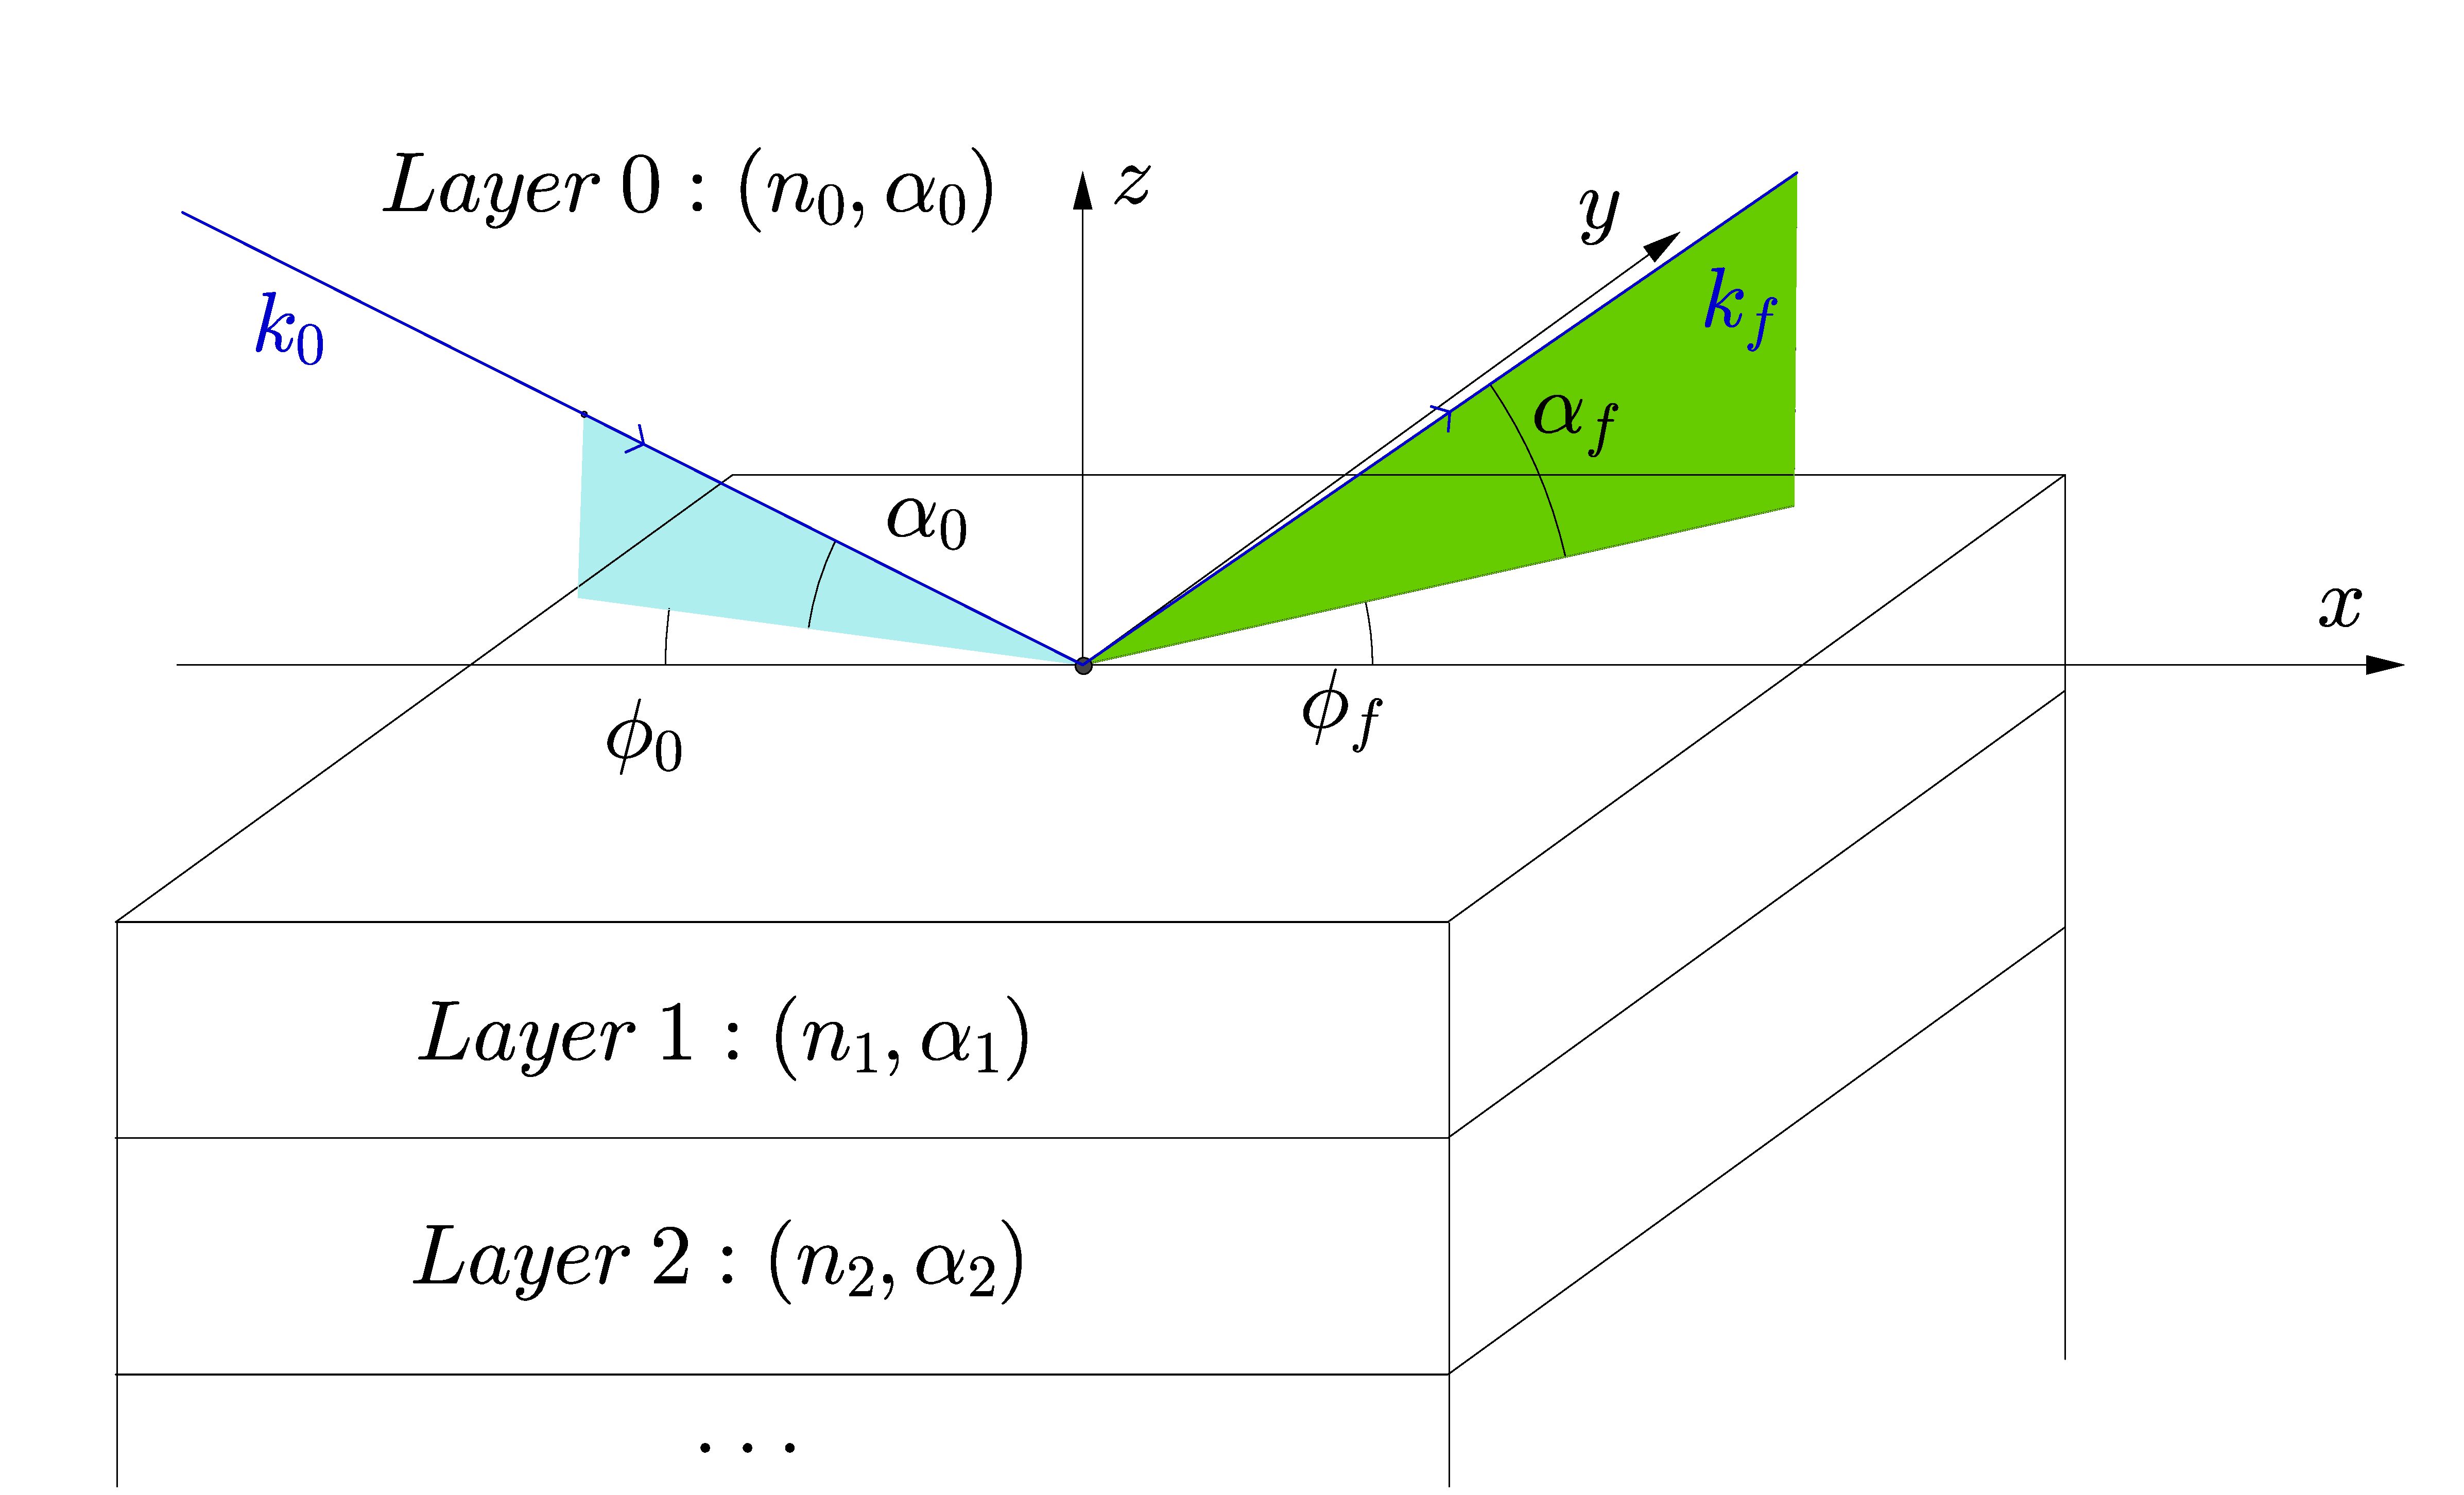
\includegraphics[clip=, width=120mm]{multilayer3d2.eps}
  \caption[Representation of the scattering geometry for multilayer
    specular reflectivity.]{Representation of the scattering geometry for multilayer
    specular reflectivity. $n_j$ is
    the refractive index of layer $j$ and $\alpha_j$ is the incident
    angle of the wave propagating in layer $j$ and incident on layer $j+1$. $\alpha_f$ is the exit angle with respect to the sample's surface and
$\phi_f$ is the scattering angle with respect to the scattering
plane. }
  \label{fig:multil3d}
\end{figure}

\noindent The input beam is assumed to be monochromatic without any
spatial divergence.\\ \textbf{polarization term?}

\subsection{Units}
By default angles are expressed in radians and lengths are given in
nanometers.  But it is possible to use other units by
specifying them right after the value of the corresponding
parameter like, for example, \texttt{20.0*Units::micrometer} in C++.


\subsection{Programs}

\MakeRemark{Programming}{The examples presented in the next
  paragraphs are written in C++ or Python. For tutorials about these
   programming languages, the users are referred to
  \cite{Cppref} and \cite{Pythonref} respectively.}\\

\noindent Note about the version of C++ and Python to run the
examples.\\

\noindent Where can the following examples be found?\\


\noindent What is the command to run the examples?

%\section{Example 1: Two types of islands on top of substrate. Nointerference function}% \sectionmark{Example 1}
\mysection{Example 1}{Example 1: Two types of islands on top of
  substrate. No interference function}% \sectionmark{Example 1}

In this example, using Python language, we simulate the scattering from a mixture of
cylindrical and prismatic nanoparticles without any interference
between them. These particles are placed in air, on top
of a substrate.\\ We are going to go through each step of the
simulation. The Python script specific to each stage will be given at
the beginning of the description. But for the sake of completeness the full code is given
at the end of this section (Listing~\ref{script_ex1}). \\

\noindent We start by importing different functions from external
modules (lines~\ref{import_begin}-\ref{import_end}). For example,
line~\ref{import_numpy}  imports NumPy, which
is a fundamental package for scientific computing with Python
(\url{http://www.numpy.org/}).  In particular, line~\ref{import_end}
imports the features of \BornAgain\ software.\\

\noindent Finally line~\ref{def_function} marks the beginning of the
function to define and run the simulation. 

\begin{lstlisting}[language=python, style=eclipseboxed,name=ex1,nolol]
import sys@\label{import_begin}@
import os
import numpy @\label{import_numpy}@

sys.path.append(os.path.abspath(os.path.join(os.path.split(__file__)[0],'..', '..', '..', 'lib')))

from libBornAgainCore import * @\label{import_end}@

def RunSimulation(): @\label{def_function}@
\end{lstlisting}


 %%%%%%%%%%%%%  
\myparagraph{\underline{First step:} Defining materials} 


\begin{lstlisting}[language=python, style=eclipseboxed,name=ex1,nolol]
#  defining materials @\label{material1}@
mAmbience = MaterialManager.getHomogeneousMaterial("Air", 0.0, 0.0 )  @\label{material2}@
mSubstrate = MaterialManager.getHomogeneousMaterial("Substrate", 6e-6, 2e-8) @\label{material3}@
\end{lstlisting}

\noindent Lines~\ref{material2} and \ref{material3} define two different
materials using function \texttt{getHomogeneousMaterial} from class
\texttt{MaterialManager}. The general syntax is the following 

\begin{lstlisting}[language=python, style=eclipse,numbers=none]
Interface material name = MaterialManager.getHomogeneousMaterial("name", delta, beta)
\end{lstlisting}

\noindent where \texttt{name} is the name of the
material associated with its complex refractive index
\texttt{n=1-delta +i beta}. \texttt{Interface material name} is later used when
referring to this particular material. The two defined materials in this example are \texttt{Air} with a refractive
index of 1 (\texttt{delta = beta =0}) and a \texttt{Substrate} associated with a complex refractive index
equal to $1-6\times 10^{-6} +i2\times 10^{-8} $. \\

\noindent \underline{Remark:} there is no condition on the choice of
\texttt{name}. 
 %%%%%%%%%%%%% 
\myparagraph{\underline{Second step:} Defining the particles} 


\begin{lstlisting}[language=python,
  style=eclipseboxed,name=ex1,nolol]
# collection of particles @\label{particles1}@
n_particle = complex(6e-4, 2e-8) @\label{complx_ref_index}@
cylinder_ff = FormFactorCylinder(5*nanometer, 5*nanometer) @\label{particlescyl1}@
cylinder = Particle(n_particle, cylinder_ff) @\label{particlescyl2}@
prism_ff = FormFactorPrism3(5*nanometer, 5*nanometer) @\label{particlesprism1}@
prism = Particle(n_particle, prism_ff) @\label{particlesprism2}@
\end{lstlisting}

 \noindent We implement two different shapes of particles: cylinders and
 prisms (\textit{i.e.} elongated particles with a constant equilateral triangular cross section).\\ All particles implemented in \BornAgain\ are defined by their
 form factors, their sizes and the refractive index of the material
  they are made of. Here, for the
  cylindrical particle, we input its radius and its height.  For the prism, 
  the possible inputs are the length of one side of its equilateral triangular
  base and its height.\\

\noindent In line~\ref{complx_ref_index}, we define the complex refractive index
associated with both particle shapes: \texttt{n}$=1-6\times 10^{-4}+i2\times 10^{-8}$.\\
  
\noindent In order to define a particle, we proceed in two steps. For example for
the cylindrical particle, we first specify the form factor of a cylinder with 
its radius and height, both equal to 5 nanometers in this particular
case (see line~\ref{particlescyl1}). Then we associate this shape with
the refractive index of the constituting material as in line~\ref{particlescyl2}.\\

\noindent The same procedure has been applied for the prism in lines~\ref{particlesprism1} and \ref{particlesprism2} respectively.
 %%%%%%%%%%%%% 
\myparagraph{\underline{Third step:} Characterizing the layers and assembling the sample} 

\noindent \textbf{Particle decoration} \\

\begin{lstlisting}[language=python, style=eclipseboxed, name=ex1,nolol]
particle_decoration = ParticleDecoration()  @\label{particlesdecor1}@
particle_decoration.addParticle(cylinder, 0.0, 0.5)  @\label{particlesdecor2}@
particle_decoration.addParticle(prism, 0.0, 0.5)@\label{particlesdecor3}@
interference = InterferenceFunctionNone()  @\label{particlesnointerf}@
particle_decoration.addInterferenceFunction(interference)  @\label{particlesinterf}@
\end{lstlisting}

\noindent The process of defining the positions and densities of particles
in our sample is called ``particle decoration''. We use the function \texttt{ParticleDecoration()}
(line~\ref{particlesdecor1}) and  the associated \texttt{addParticle}
for each particle shape (lines~\ref{particlesdecor2}, \ref{particlesdecor3}). The general
syntax is 

\begin{lstlisting}[language=python, style=eclipse,numbers=none]
particledecoration.addParticle(particle_name, depth, abundance) 
\end{lstlisting}

\noindent  where \texttt{particle\_name} is the name used to define the particles
(lines~\ref{particlescyl2} and \ref{particlesprism2}), \texttt{depth}
(default value =0)
is the vertical position, expressed in nanometers, of the particles in a given layer (the
association with a particular layer will be done during the next step) and
\texttt{abundance} is the proportion of this type of particles, 
normalized to the total number of particles. Here we have 50\% of cylinders
and 50\% of prisms. \\ 

\noindent {\huge\danger} 
\colorbox{Lightgray}{\parbox{\dimexpr\linewidth-8\fboxsep}
{\underline{Remark -} Depth of particles\\
The vertical positions of particles in a layer are given in relative
coordinates. For the top layer, the bottom corresponds to
\texttt{depth}=0 and negative values would correspond to particles
floating above layer 1 since the vertical axis, shown in
fig.~\ref{fig:multil3d} is pointing upwards. But for all the other layers, it is the top of the
layer which corresponds to \texttt{depth}=0.}}\\


\noindent Finally lines~\ref{particlesnointerf} and
\ref{particlesinterf} specify that there is \textbf{no coherent interference} between
the waves scattered by these particles. The intensity is calculated by
the incoherent sum of the scattered waves: $\langle |F_n|^2\rangle$,
where $F_n$ is the form factor associated with the particle of type $n$.  The way these waves
interfere imposes the horizontal distribution of
the particles as
the interference reflects the long or short-range order of the
particles distribution (\textbf{see Theory}). On the contrary, the vertical position is
imposed when we add the particles in a given layer by parameter \texttt{depth}, as shown in lines~\ref{particlesdecor2} and \ref{particlesdecor3}. \\

\noindent \textbf{Multilayer}\\

\begin{lstlisting}[language=python, style=eclipseboxed,name=ex1,nolol]
# air layer with particles and substrate form multi layer  @\label{sampleassembling}@
air_layer = Layer(mAmbience)  @\label{airlayer}@
air_layer_decorator = LayerDecorator(air_layer, particle_decoration)  @\label{airlayerdecorator}@
substrate_layer = Layer(mSubstrate, 0)  @\label{substratelayer}@
multi_layer = MultiLayer()  @\label{multilayercanvas}@
multi_layer.addLayer(air_layer_decorator)  @\label{layerairdecor}@
multi_layer.addLayer(substrate_layer)  @\label{layersubstrate}@
\end{lstlisting}

\noindent We now have to configure our sample. For this first example,
the particles, \textit{i.e.} cylinders and prisms, are on top of a substrate in an
air layer. \textbf{The order in which we define these layers is important: we
start from the top layer down to the bottom one}.\\

\noindent Let us start with the air layer. It contains the particles. In
line~\ref{airlayer}, we use the previously defined \texttt{mAmbience}
(="air" material) (line~\ref{material2}). The command written in line~\ref{airlayerdecorator} shows that this layer is decorated by adding the
particles using the function \texttt{particledecoration} defined in
lines~\ref{particlesdecor1}-\ref{particlesinterf}. Note that the
\texttt{depth} is referenced to the bottom of the top layer (negative
values would correspond to particles floating above layer 1 as
the vertical axis is pointing upwards). The substrate layer
only contains the substrate material (line~\ref{substratelayer}).\\
 
\noindent There are different possible syntaxes to define a layer. As shown in
lines~\ref{airlayer} and \ref{substratelayer}, we can use
\texttt{Layer(Interface material name,thickness)} or
\texttt{Layer(Interface material name)}. The second case corresponds
to the default value of the \texttt{thickness}, equal to 0. The \texttt{thickness} is
expressed in  nanometers. \\

\noindent Our two layers are now fully characterized. The sample is assembled using
\texttt{MultiLayer()} constructor (line~\ref{multilayercanvas}): we start with the air layer decorated
with the particles (line~\ref{layerairdecor}), which is the layer at
the top and end with the bottom layer, which is the
substrate (line~\ref{layersubstrate}).
 %%%%%%%%%%%%% 
\myparagraph{\underline{Fourth step:} Characterizing the input beam and
output detector and running the simulation} 


\begin{lstlisting}[language=python, style=eclipseboxed,name=ex1,nolol]
# run simulation  @\label{run1}@
simulation = Simulation()  @\label{run2}@
simulation.setDetectorParameters(100,-1.0*degree, 1.0*degree, 
                                100, 0.0*degree, 2.0*degree, True)  @\label{rundetector}@
simulation.setBeamParameters(1.0*angstrom, 0.2*degree, 0.0*degree)  @\label{runbeam}@
simulation.setSample(multi_layer)  @\label{runsample}@
simulation.runSimulation()  @\label{runsimul}@
\end{lstlisting}


\noindent The first stage is to define the \texttt{Simulation()} object (line~\ref{run2}). Then we define the detector (line~\ref{rundetector}) and beam
parameters (line~\ref{runbeam}), which are associated with the
sample previously defined (line~\ref{runsample}). Finally we run
the simulation (line~\ref{runsimul}). Those functions are part of the Simulation
class.  The
different incident and exit angles are
shown in Fig.~\ref{fig:multil3d}. \\

\noindent The detector parameters are set using ranges of angles via
the function:\\

\noindent \texttt{setDetectorParameters(n\_phi, phi\_f\_min,
  phi\_f\_max,\\ \phantom{setDetectorParameters(}n\_alpha, alpha\_f\_min, alpha\_f\_max, isgisaxs\_style=false)}, \\

\noindent where \texttt{n\_phi=100} is the number of points in the range of
variations of angle $\phi_f$,\\ \texttt{phi\_f\_min=-1.0*degree} and \texttt{phi\_f\_max=1.0*degree}
are the minimum and maximum values respectively of $\phi_f$, which is the in-plane direction of the scattered beam
(measured with respect to the $x$-axis), \\ \texttt{n\_alpha=100} is
the number of points in the range of variations of the exit angle
$\alpha_f$ measured from the $x,y$-plane in the $z$-direction,\\ \texttt{alpha\_f\_min=0.0*degree} and \texttt{alpha\_f\_max=2.0*degree} 
are the minimum and maximum values respectively of $\alpha_f$,\\
\texttt{isgisaxs\_style=True} (default value = \texttt{False}) is a boolean
used to characterise the structure of the output data. If
\texttt{isgisaxs\_style=True}, the output data is binned at constant
values of the sine of the output angles, $\alpha_f$ and $\phi_f$, otherwise it is binned
at constant values of these two angles.\\


\noindent For the beam the function to use is
\texttt{simulation.setBeamParameters(lambda, alpha\_i, phi\_i)}, where
\texttt{lambda=1.0*angstrom} is the incident beam wavelength,\\
\texttt{alpha\_i=0.2*degree} is the incident
grazing angle on the surface of the sample,
\texttt{phi\_i=0.0*degree} is the in-plane
direction of the incident beam (measured with respect to the
$x$-axis). Note that in Fig.~\ref{fig:multil3d} $\alpha_i=\alpha_0$ and $\phi_i=\phi_0$.\\ 

\noindent \underline{Remark}: Note that, except for
\texttt{isgisaxs\_style}, there are no default values implemented for the
parameters of the beam and detector.\\

\noindent Line~\ref{runsimul} shows the command to run the simulation using the
previously defined setup.
%%%%%%%%%%%%%
\myparagraph{\underline{Fifth step:} Saving the data} 


\begin{lstlisting}[language=python, style=eclipseboxed,name=ex1,nolol]
# retrieving intensity data
return GetOutputData(simulation) @\label{outputdata}@%arr = GetOutputData(simulation) @\label{outputdata}@
\end{lstlisting}


\noindent In line~\ref{outputdata} we record the simulated intensity
as a function of outgoing angles $\alpha_f$ and $\phi_f$ for further
uses (plots, fits,\ldots) as a NumPy array containing
\texttt{n\_phi}$\times$\texttt{n\_alpha}
datapoints. Some options are provided by \BornAgain. For example, figure~\ref{fig:output_ex1} shows the two-dimensional
contourplot of the intensity as a function of $\alpha_f$ and
$\phi_f$. 

\begin{figure}[h]
  \begin{center}
   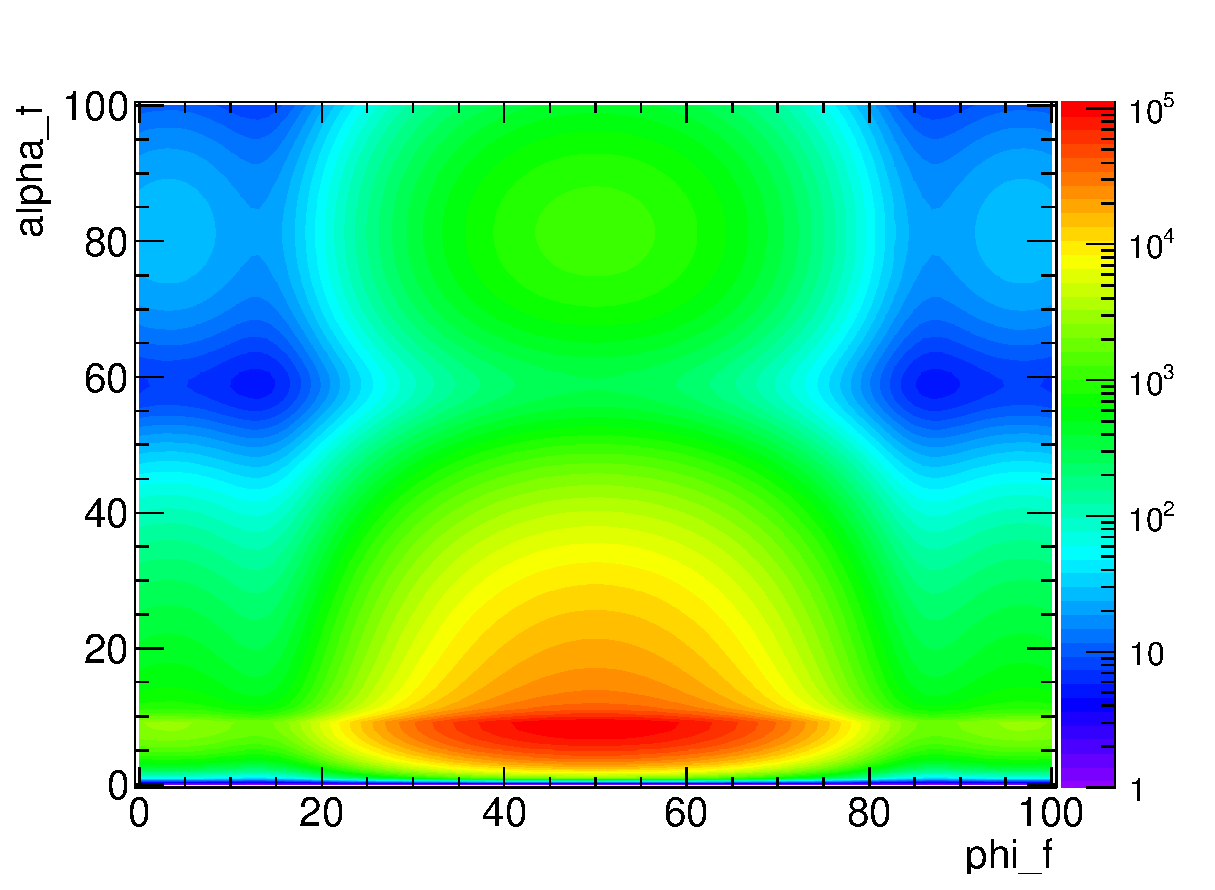
\includegraphics[clip=true, width=120mm]{Manual_ex1.eps}
  \end{center}
  \caption[Example 1: Simulated grazing-incidence small-angle X-ray scattering from a mixture of
cylindrical and prismatic nanoparticles without any interference, deposited on top
of a substrate]{Figure of example 1: Simulated grazing-incidence small-angle X-ray scattering from a mixture of
cylindrical and prismatic nanoparticles without any interference, deposited on top
of a substrate. The input beam is characterized by a wavelength
$\lambda$ of 1~\AA\ and incident angles $\alpha_i=0.2^{\circ}$, $\phi_i=0^{\circ}$. The
cylinders have a radius and a height both equal to 5~nm, the prisms
are characterized by a side length equal to 5~nm and they are also 5~nm high. The
material of the particles has a refractive index of $1-6\times 10^{-4}+i2\times 10^{-8}$. For the substrate
it is equal to $1-6\times 10^{-6} +i2\times 10^{-8} $. The colorscale
is associated with the output intensity in arbitrary units. }
\label{fig:output_ex1}
\end{figure}

\newpage
\begin{lstlisting}[caption={Python script of example 1},
  label=script_ex1,captionpos=b,escapeinside={@}{@} ,language=python,style=eclipse, numbers= none,frame = leftline ,
      framerule = 2mm ,
      rulecolor = \color{lightgrey},
      breaklines = true]
import sys
import os
import numpy 

sys.path.append(os.path.abspath(os.path.join(os.path.split(__file__)[0],'..', '..', '..', 'lib')))

from libBornAgainCore import * 

def RunSimulation():
    #  defining materials 
    mAmbience = MaterialManager.getHomogeneousMaterial("Air", 0.0, 0.0 ) 
    mSubstrate = MaterialManager.getHomogeneousMaterial("Substrate", 6e-6, 2e-8) 
    # collection of particles 
    n_particle = complex(6e-4, 2e-8) 
    cylinder_ff = FormFactorCylinder(5*nanometer, 5*nanometer) 
    cylinder = Particle(n_particle, cylinder_ff) 
    prism_ff = FormFactorPrism3(5*nanometer, 5*nanometer) 
    prism = Particle(n_particle, prism_ff) 
    particle_decoration = ParticleDecoration()  
    particle_decoration.addParticle(cylinder, 0.0, 0.5)  
    particle_decoration.addParticle(prism, 0.0, 0.5)  
    interference = InterferenceFunctionNone()  
    particle_decoration.addInterferenceFunction(interference)  
    # air layer with particles and substrate form multi layer 
    air_layer = Layer(mAmbience)  
    air_layer_decorator = LayerDecorator(air_layer, particle_decoration) 
    substrate_layer = Layer(mSubstrate, 0) 
    multi_layer = MultiLayer()  
    multi_layer.addLayer(air_layer_decorator) 
    multi_layer.addLayer(substrate_layer) 

    # run simulation  
    simulation = Simulation()  
    simulation.setDetectorParameters(100,-1.0*degree, 1.0*degree, 
                                    100, 0.0*degree, 2.0*degree, True) 
    simulation.setBeamParameters(1.0*angstrom, 0.2*degree, 0.0*degree) 
    simulation.setSample(multi_layer) 
    simulation.runSimulation()  

    # retrieving intensity data
     return GetOutputData(simulation)
\end{lstlisting}



% \newpage
% \subsection{Hello, minted}
% 
% \begin{minted}[linenos=true, frame=single]{python}
% mAmbience = MaterialManager.getHomogeneousMaterial("Air", 1.0, 0.0 )
% mSubstrate = MaterialManager.getHomogeneousMaterial("Substrate", 1.0-6e-6, 2e-8 )
% n_particle = complex(1.0-6e-4, 2e-8)
% cylinder_ff = FormFactorCylinder(5*nanometer, 5*nanometer)
% cylinder = Particle(n_particle, cylinder_ff)
% prism_ff = FormFactorPrism3(5*nanometer, 5*nanometer)
% prism = Particle(n_particle, prism_ff)
% particle_decoration = ParticleDecoration()
% particle_decoration.addParticle(cylinder, 0.0, 0.5)
% particle_decoration.addParticle(prism, 0.0, 0.5)
% interference = InterferenceFunctionNone()
% particle_decoration.addInterferenceFunction(interference)
% # air layer with particles and substrate form multi layer
% air_layer = Layer(mAmbience)
% air_layer_decorator = LayerDecorator(air_layer, particle_decoration)
% substrate_layer = Layer(mSubstrate, 0)
% multi_layer = MultiLayer()
% multi_layer.addLayer(air_layer_decorator)
% multi_layer.addLayer(substrate_layer)
% 
% # build and run experiment
% simulation = Simulation()
% simulation.setDetectorParameters(100,-1.0*degree, 1.0*degree, 100, 0.0*degree, 2.0*degree, True)
% simulation.setBeamParameters(1.0*angstrom, -0.2*degree, 0.0*degree)
% simulation.setSample(multi_layer)
% simulation.runSimulation()
% \end{minted}

\section{Example 2}



